\documentclass[]{book}
\usepackage{lmodern}
\usepackage{amssymb,amsmath}
\usepackage{ifxetex,ifluatex}
\usepackage{fixltx2e} % provides \textsubscript
\ifnum 0\ifxetex 1\fi\ifluatex 1\fi=0 % if pdftex
  \usepackage[T1]{fontenc}
  \usepackage[utf8]{inputenc}
\else % if luatex or xelatex
  \ifxetex
    \usepackage{mathspec}
  \else
    \usepackage{fontspec}
  \fi
  \defaultfontfeatures{Ligatures=TeX,Scale=MatchLowercase}
\fi
% use upquote if available, for straight quotes in verbatim environments
\IfFileExists{upquote.sty}{\usepackage{upquote}}{}
% use microtype if available
\IfFileExists{microtype.sty}{%
\usepackage{microtype}
\UseMicrotypeSet[protrusion]{basicmath} % disable protrusion for tt fonts
}{}
\usepackage[margin=1in]{geometry}
\usepackage{hyperref}
\hypersetup{unicode=true,
            pdftitle={Style Guide for Loss Data Analytics},
            pdfauthor={An open text authored by the Actuarial Community},
            pdfborder={0 0 0},
            breaklinks=true}
\urlstyle{same}  % don't use monospace font for urls
\usepackage{natbib}
\bibliographystyle{apalike}
\usepackage{longtable,booktabs}
\usepackage{graphicx,grffile}
\makeatletter
\def\maxwidth{\ifdim\Gin@nat@width>\linewidth\linewidth\else\Gin@nat@width\fi}
\def\maxheight{\ifdim\Gin@nat@height>\textheight\textheight\else\Gin@nat@height\fi}
\makeatother
% Scale images if necessary, so that they will not overflow the page
% margins by default, and it is still possible to overwrite the defaults
% using explicit options in \includegraphics[width, height, ...]{}
\setkeys{Gin}{width=\maxwidth,height=\maxheight,keepaspectratio}
\IfFileExists{parskip.sty}{%
\usepackage{parskip}
}{% else
\setlength{\parindent}{0pt}
\setlength{\parskip}{6pt plus 2pt minus 1pt}
}
\setlength{\emergencystretch}{3em}  % prevent overfull lines
\providecommand{\tightlist}{%
  \setlength{\itemsep}{0pt}\setlength{\parskip}{0pt}}
\setcounter{secnumdepth}{5}
% Redefines (sub)paragraphs to behave more like sections
\ifx\paragraph\undefined\else
\let\oldparagraph\paragraph
\renewcommand{\paragraph}[1]{\oldparagraph{#1}\mbox{}}
\fi
\ifx\subparagraph\undefined\else
\let\oldsubparagraph\subparagraph
\renewcommand{\subparagraph}[1]{\oldsubparagraph{#1}\mbox{}}
\fi

%%% Use protect on footnotes to avoid problems with footnotes in titles
\let\rmarkdownfootnote\footnote%
\def\footnote{\protect\rmarkdownfootnote}

%%% Change title format to be more compact
\usepackage{titling}

% Create subtitle command for use in maketitle
\newcommand{\subtitle}[1]{
  \posttitle{
    \begin{center}\large#1\end{center}
    }
}

\setlength{\droptitle}{-2em}
  \title{Style Guide for Loss Data Analytics}
  \pretitle{\vspace{\droptitle}\centering\huge}
  \posttitle{\par}
  \author{An open text authored by the Actuarial Community}
  \preauthor{\centering\large\emph}
  \postauthor{\par}
  \predate{\centering\large\emph}
  \postdate{\par}
  \date{2018-09-01}

\usepackage{booktabs}
\usepackage{hyperref}
\hypersetup{colorlinks,%
citecolor=blue,%
linkcolor=blue,%
urlcolor=blue,%
pdftex}

\usepackage{amsthm}
\newtheorem{theorem}{Theorem}[chapter]
\newtheorem{lemma}{Lemma}[chapter]
\theoremstyle{definition}
\newtheorem{definition}{Definition}[chapter]
\newtheorem{corollary}{Corollary}[chapter]
\newtheorem{proposition}{Proposition}[chapter]
\theoremstyle{definition}
\newtheorem{example}{Example}[chapter]
\theoremstyle{definition}
\newtheorem{exercise}{Exercise}[chapter]
\theoremstyle{remark}
\newtheorem*{remark}{Remark}
\newtheorem*{solution}{Solution}
\begin{document}
\maketitle

{
\setcounter{tocdepth}{1}
\tableofcontents
}
\chapter*{Preface}\label{preface}
\addcontentsline{toc}{chapter}{Preface}

It is important for chapters in the \emph{Open Actuarial Textbooks}
project to have a consistent look and feel. The \emph{Style Guide for
Loss Data Analytics} aims to assist contributors in developing chapters
consistently throughout the \emph{Loss Data Analytics} book.

This guide is set up as sample chapters containing

\begin{itemize}
\tightlist
\item
  information regarding suitable content for a chapter,
\item
  methods to implement chapter elements and
\item
  conventions for consistent notation.
\end{itemize}

\chapter{Chapter Structure}\label{chapter-structure}

\begin{center}\rule{0.5\linewidth}{\linethickness}\end{center}

In this chapter, you learn how to:

\begin{itemize}
\tightlist
\item
  Determine what and what not to include in a chapter
\item
  Include technical supplements as needed
\item
  Assess types of exercises and book resources that are appropriate for
  a chapter
\end{itemize}

\begin{center}\rule{0.5\linewidth}{\linethickness}\end{center}

\section{Chapter Preview and Learning
Objectives}\label{chapter-preview-and-learning-objectives}

\begin{itemize}
\item
  \emph{Chapter Preview}. Begin with a chapter preview to set the stage
  of the chapter.
\item
  \emph{Learning Objectives}. At the beginning of each chapter and
  section, describe in a few bullet points what the reader can expect to
  learn.
\end{itemize}

\section{Main Body}\label{main-body}

Split the chapter into 4-7 sections; within each section, introduce 0-5
subsections. Do not develop a deeper hierarchy (e.g., a
``sub-subsection''). Use nonlinear aspects of the web. For example,
detailed mathematical developments can go into a technical appendix or
are simply hidden (using javascript ``hide/show'' tools) unless the
viewer really wants to see the details. Case studies and historical
references can be included in ``side-bars,'' a supporting webpage. For
the main body of the chapter, think about ``25 pages'' in length
(whatever that means\ldots{}.).

\subsection{What to Include}\label{what-to-include}

\begin{itemize}
\item
  Within the chapter, use boxed and numbered lists of procedures for
  easy reference.
\item
  It is certainly okay (and expected) to use mathematical notation
  although please adhere to the conventions described in Section
  \ref{S:NotationConvention}. Each chapter should have examples
  interwoven within theory, allowing readers to see the development of
  the theory along with the importance of the applications.
\item
  Distinguish between an \emph{``Example''} and a \emph{``Special
  Case''}. The former shows how to relate the mathematics to a practical
  situation likely to be encountered by a practicing actuary. The latter
  looks at a subset of a general (usually) mathematical result. A few
  special cases are certainly acceptable but we want to focus on
  developing examples.
\item
  Think of graphical ways to visualize/summarize relationships that you
  want to emphasize.
\item
  Begin each section with a short bullet list describing the learning
  objectives of that section. Finish each section with a short quiz on
  these learning objectives. As of this writing (July 2018), quizzes are
  multiple-choice.
\item
  Include short exercises/examples/special cases that can be readily
  solved by the viewer (with solutions using ``hide/show'' features)
  within the main body. These serve to reinforce concepts and provide
  benchmarks for understanding.
\end{itemize}

\subsection{What Not to Include}\label{what-not-to-include}

\begin{itemize}
\item
  Do not include development of equations/formulas in the main body of
  the text. The main body of the text will be devoted to presenting
  results, providing context and intuition as to the importance of the
  results.
\item
  Do not include references to the literature. This will appear in the
  last section on ``Further Reading and References.''
\item
  Do not include graphs whose information could easily be summarized by
  a table.
\end{itemize}

\section{Technical Supplements}\label{technical-supplements}

We want our viewers to understand the underpinnings of the theory (the
old analogy of ``what is going on under the hood to see how the engine
works'' - no black boxes.) So, there will be occasions when you feel
like a short development or ``proof''; is reasonable. Put this in an
appendix. Technical supplements should develop the theory in a
step-by-step fashion, building on each concept in a crisp, mathematical
fashion.

\section{Contributors and Further
Resources}\label{S:further-reading-and-resources}

\subsection{Contributors}\label{contributors}

Make sure that contributors are listed at the end of the chapter. The
following provides an example.

\begin{verbatim}
####Contributors {-}

- Edward W. (Jed) Frees, University of Wisconsin-Madison, 
is the principal author of the initital version of this chapter. 
Email: jfrees@bus.wisc.edu for chapter comments and 
suggested improvements. Helpful improvements provided by
Alyaa Nuval Binti Othman and Aisha Nuval Binti Othman.
\end{verbatim}

\subsection{Further Reading and
References}\label{further-reading-and-references}

Do not finish with a ``preview of upcoming chapter''; finish instead
with a ``Further Reading and References.'' This consists of a series of
references with one or two lines of annotation for each reference that
the interested reader could follow up on (self-citations are okay!).
Historical developments are particularly nice in this section.

\chapter{Interactive Book Features}\label{S:Interactive}

An advantage of publishing on the web is that we can produce an online
version that contains many interactive objects such as quizzes, computer
demonstrations, interactive graphs, video, and the like, to promote
\textbf{deeper learning}.

We want viewers to interact with the book; it is \textbf{not} written to
accommodate the ``armchair reader,'' that is, one who passively reads
and does not get involved by attempting the exercises in the text.
Consider an analogy to sports; there is a great deal that you can learn
about the game just by watching. However, if you want to sharpen your
skills, then you have to go out and play the game.

\section{Examples and Exercises}\label{examples-and-exercises}

Even for traditional offline (pdf) version of the book, we include
problems that allow readers to develop their learning.

Each chapter contains several ``Examples'' or ``Exercises'' - these are
focused problems that generally ask the reader to do a calculation or
provide an interpretation of a statistical issue. We call them
``examples'' when they appear in the main body of the text and
``exercises'' when they appear at the end of the chapter. The need for
hand calculations has been advocated by Khamis (1991)\footnote{``Manual
  Computations---A Tool for Reinforcing Concepts and Techniques,'' H. J.
  Khamis, Pages 294-299, \emph{The American Statistician}, Volume 45,
  1991 - Issue 4}. Many teachers have found it useful to practice the
mechanics in order to provide a solid foundation. With this foundation,
we can get on to the real business; interpreting data using statistical
principles.

We anticipate that substantial exercise banks will be built over time by
users, professional associations, and those with commercial interests.
When developing the chapter foundations, think about the following types
of problems.

\begin{itemize}
\tightlist
\item
  \textbf{Hand Calculation.} These are problems that can be solved
  without the use of a computer. They typically reinforce a statistical
  or actuarial concept as well as highlight an issue that might be
  encountered in practice. For this book, these problems often involve
  algebraic and calculus manipulations. When writing these types of
  problems, readers are more motivated if they understand \emph{why} the
  problem is important. What actuarial issue is being addressed? What
  statistical concept is being practiced? Often, a simple line or two
  prefacing a problem can help substantially in this regard.
\item
  \textbf{Software.} These are problems that ask the reader to work with
  \texttt{R} software, such as calculating a function or reproducing a
  graph.
\item
  \textbf{Data.} These are problems that ask the reader to work with
  data. The need for working with real data is well documented; for
  example, see Hogg (1972), Moore and Roberts (1989) or Singer and
  Willett (1990). By providing detailed guided tutorials that work with
  theory and data, we teach our students the essence of \emph{Loss Data
  Analytics}. Of course, there are some important disadvantages to
  working with real data. Data sets can quickly become outdated.
  Further, the ideal data set to illustrate a specific statistical issue
  is difficult to find. Data exercises are complex and can span several
  chapter sections as well as chapters.
\end{itemize}

Examples and exercises are designed so that they illustrate a general
analytics/statistical concept; they have the additional advantage in
that they are often based on actuarial professional examinations and so
provide readers with training for these assessment frameworks. Notably,
\emph{in the online version of the book, the solutions to the examples
and exercises are hidden to encourage readers to actively solve (or at
least consider) prior to revealing a solution.}

\section{Statistical Code}\label{statistical-code}

However, the limitation of exercise and examples done by hand is that
they give \textbf{little insight} as to how the general
analytics/statistical concepts can be used in applications or why more
extensive treatments beyond the foundations would be needed. To address
these limitations, throughout we include illustrate statistical code
with sample (but real) datasets. The statistical language used
throughout is \texttt{R}. For two reasons, the \texttt{R} code is hidden
in the online version but can be interactively revealed but clicking a
button.

\begin{itemize}
\tightlist
\item
  First, we want to focus on the analytics/statistical concepts and do
  not wish for readers to be distracted by software code that emphasizes
  implementation, not concepts.
\item
  Second, not all readers will use \texttt{R} (there are many good
  alternative software programs available) and we want the book to be
  available to a broad readership.
\end{itemize}

Although we do not focus on developing \texttt{R} tutorials, we will
provide guides and links to people who wish to learn \texttt{R}. Our
focus is on teaching statistical methods and actuarial issues, not
software. Over time, the project may also provide support for users of
other software environments, such as Microsoft's Excel or Python.

\section{Other Interactive Features}\label{other-interactive-features}

A wonderful aspect of an online text is that we can readily incorporate
other interactive features. In coming versions of the book, you can
expect to see

\begin{itemize}
\tightlist
\item
  a glossary (hover the cursor over a technical word or phrase to reveal
  a definition),
\item
  links to relevant applications of the basic concept, as well as
\item
  end of the section quizzes that provide ``low-level formative
  assessments'' so that they reader can gauge his or her understanding
  of the material.
\end{itemize}

Some of the support material associated with the book also emphasizes
interactive aspects. For example, detailed \emph{R code} allows readers
to learn complex statistical routines and provides sample code so that
users can develop their own libraries of useful routines. Another site
will feature \texttt{R-Shiny}, an interactive graphic tool that provides
dynamic graphing features. The concept of active learning promotes one
of the deeper learning goals set forth by some educational leaders: The
ability to learn how to learn independently.

\section{Additional Book Resources Supporting Each
Chapter}\label{additional-book-resources-supporting-each-chapter}

We are hopeful that there will be several resources support the book
that will appear outside of the chapter structure. Although not
necessarily interactive, they will help develop users' learning. These
include:

\begin{itemize}
\tightlist
\item
  \textbf{Case Studies and Historical Vignettes.} Similar to those
  appearing within the chapter, include short exercises/examples/special
  cases that can be readily solved by the viewer. These serve to
  reinforce concepts and provide benchmarks for understanding. Case
  studies can be used to emphasize different practices in different
  countries. Historical vignettes can be interesting in their own right
  and remind us all of the foundations of our discipline.
\item
  \textbf{Data.} We anticipate developing a library of data sets that
  can be used by instructors who wish to emphasize different areas of
  practice.
\item
  \textbf{Technical Supplements, Lists, and Tables.} The roles of
  technical supplements has already been described and there could be
  many. As is common in textbooks, we will also provide a place for
  lists or tables of organized facts for learners.
\end{itemize}

\chapter{\texorpdfstring{Samples of Writing in
\texttt{R\ bookdown}}{Samples of Writing in R bookdown}}\label{S:SampleSection}

\begin{center}\rule{0.5\linewidth}{\linethickness}\end{center}

In this chapter, you learn how to:

\begin{itemize}
\tightlist
\item
  Reference other sections and equations
\item
  Include in-text citation that links to the bibliography
\item
  Include tables and figures not generated by \texttt{R} code
\item
  Include a footnote
\end{itemize}

\begin{center}\rule{0.5\linewidth}{\linethickness}\end{center}

As we expand our contributor and reviewer base, it will be helpful to
know more about the conventions used in the series regarding the details
of \texttt{R\ markdown} and \texttt{R\ bookdown} used in the series.
This chapter summarizes these conventions.

\section{Section Labels and Learning Objectives}\label{S:SectionLabels}

The following shows how to code Section titles and refer to them.

\begin{verbatim}
## Section Labels {#S:SectionLabels}
\end{verbatim}

With that reference, one can readily refer to Section
\ref{S:SectionLabels} in your text, as follows:

\begin{verbatim}
With that reference, one can readily refer to 
Section \\ref{S:SectionLabels} in your text, as follows:
\end{verbatim}

The following shows how to code learning objectives:

\begin{verbatim}
***
In this chapter, you learn how to:
  
- Reference other sections and equations
- Include in-text citation that links to the bibliography
- Include tables and figures
- Include a footnote

***

\end{verbatim}

\section{Equation References}\label{equation-references}

Here is an example of a latex equation produced in \texttt{R\ markdown},
with reference number.

\begin{equation}
  x + y = 1  
\label{eq:ExampleEquation}
\end{equation}

You can produce that equation using the following code.

\begin{verbatim}
\begin{equation}
  x + y = 1  
\label{eq:ExampleEquation}
\end{equation}
\end{verbatim}

With this, equation \eqref{eq:ExampleEquation} can be referred to using
the following code:

\begin{verbatim}
With this, equation \\eqref{eq:ExampleEquation} can be 
referred to using the following code:
\end{verbatim}

\section{In-text Citations}\label{in-text-citations}

Here is an example of an in-text citation made possible by
\texttt{R\ bookdown} \citep{xie2015}. This links to the bibliography
where the full referece is displayed. As a convention we use the
\emph{APA} style citation.

\begin{verbatim}
Here is an example of an in-text citation made possible by 
`R bookdown` [@xie2015]. This links to the bibliography 
where the full reference is displayed. 
As a convention we use the *APA* style citation.
    
\end{verbatim}

\section{Including Tables}\label{including-tables}

In order to include table not generated by \texttt{R} such as a Latex
table, we have to make some adjustments to regular Latex syntax.

\[
\begin{matrix}
    \begin{array}{c|c} \hline
    \text{Policyholder} & \text{Number of claims} \\\hline
    \textbf{X} & 1 \\\hline
    \textbf{Y} & 2 \\\hline
    \end{array}
\end{matrix}
\]

\protect\hyperlink{tab:2.1}{Table 2.1} : An example of including tables
using Latex in an \texttt{R\ markdown} document

\texttt{R\ markdown} does not have a convention for referencing non-R
generated tables. For now, we reference them manually as in refer to
\protect\hyperlink{tab:2.1}{Table 2.1}. We do this by manually inserting
an html anchor tag.

The following code produces this table.

\begin{verbatim}
<a id=tab:2.1></a> 

[Table 2.1]: \#tab:2.1

$$
\begin{matrix}
    \begin{array}{c|c} \hline
    \text{Policyholder} & \text{Number of claims} \\\hline
    \textbf{X} & 1 \\\hline
    \textbf{Y} & 2 \\\hline
    \end{array}
\end{matrix}
$$
    
[Table 2.1] : An example of including tables using Latex in an `R markdown` document    

    
\end{verbatim}

For reference, then use

\begin{verbatim}

`R markdown` does not have a convention for referencing 
non-R generated tables. For now, we reference them manually 
as in refer to [Table 2.1].
\end{verbatim}

\section{Including Figures}\label{including-figures}

\subsection{\texorpdfstring{Figures Generated by
\texttt{R}}{Figures Generated by R}}\label{figures-generated-by-r}

Most figures are generated using \texttt{R}. Here is an illustrative
figure.

\begin{figure}

{\centering 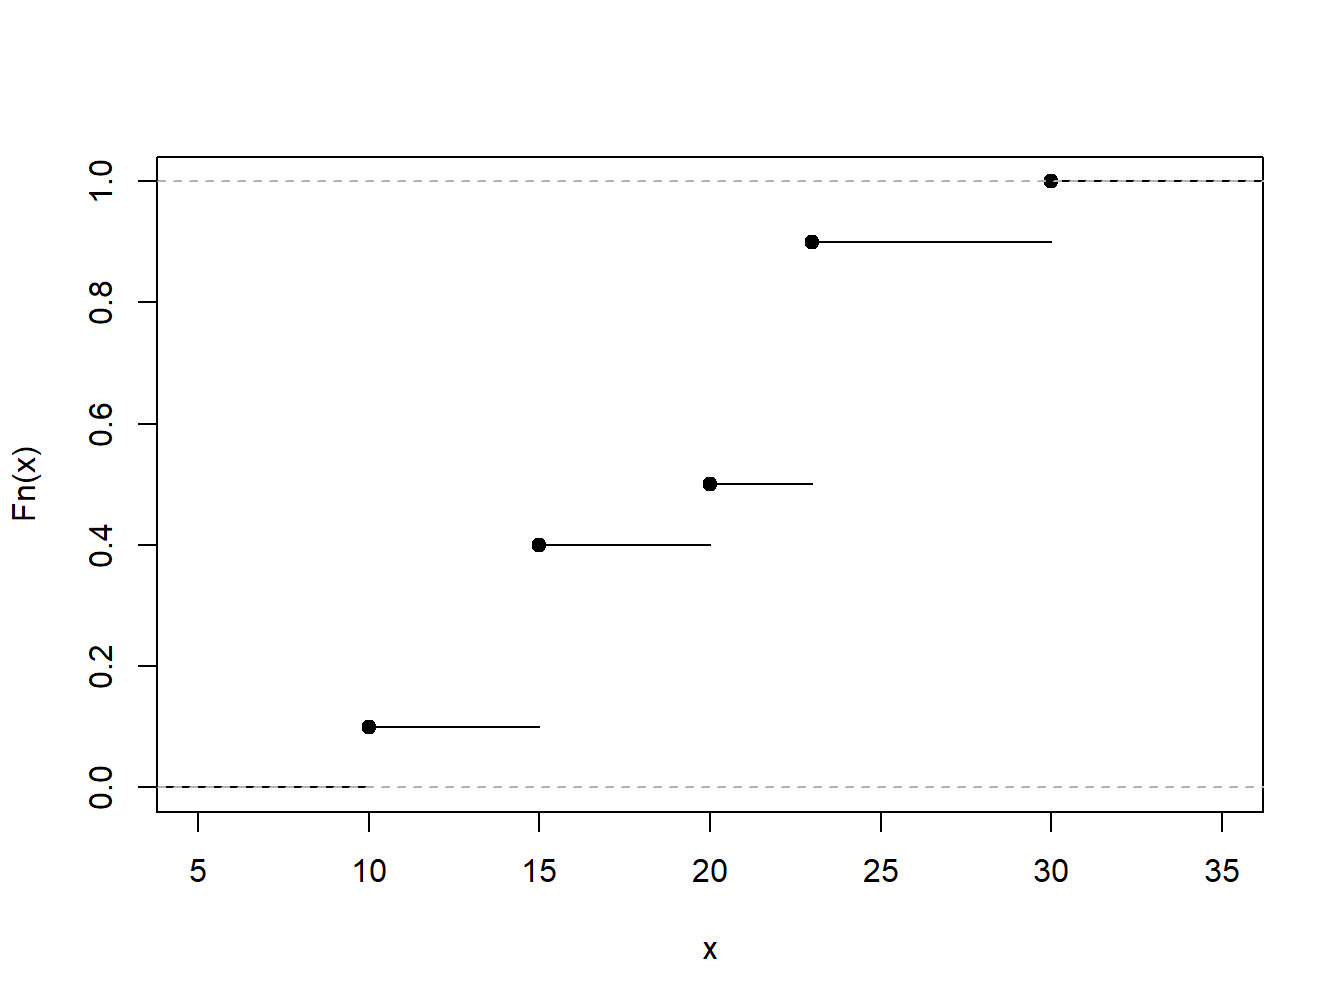
\includegraphics[width=0.6\linewidth]{Style_Guide_for_LDA_files/figure-latex/EDFToy-1} 

}

\caption{Empirical Distribution Function of a Toy Example}\label{fig:EDFToy}
\end{figure}

that we refer to as Figure \ref{fig:EDFToy}. Here is the code for
producing the figure:

\begin{verbatim}
```{r EDFToy, echo = FALSE, 
   fig.cap = 'Empirical Distribution Function of a Toy Example',
   out.width = '60%', fig.asp = 0.75, fig.align = 'center'}
xExample <- c(10,rep(15,3),20,rep(23,4),30)
PercentilesxExample <- ecdf(xExample)
plot(PercentilesxExample, main = "", xlab = "x")
```
\end{verbatim}

Here is is the code for referencing the Figure \ref{fig:EDFToy}:

\begin{verbatim}
Here is is the code for referencing the Figure \\ref{fig:EDFToy}:
    
\end{verbatim}

\subsection{\texorpdfstring{Figures Not Generated by
\texttt{R}}{Figures Not Generated by R}}\label{figures-not-generated-by-r}

For figures, we store the figures as png or jpeg files in a separate
folder called ``Figures''. Then we use \texttt{R} code to call those
figures for display so that we can reference them.

Here is such a figure:

\begin{figure}

{\centering 
\includegraphics[width=0.05\linewidth]{Figures/RStudio-Ball} 

}

\caption{An example of including figures in an R Markdown document}\label{fig:ExampleFigure}
\end{figure}

And here is the code that generates the figure:

\begin{verbatim}
"three backticks"{r, ExampleFigure, fig.cap = 'An example 
of including figures in an R Markdown document', 
out.width = '5%', fig.align = 'center', echo = FALSE}
knitr::include_graphics("Figures/RStudio-Ball.png")
"three backticks"
\end{verbatim}

Here is is the code for referencing the Figure \ref{fig:ExampleFigure}:

\begin{verbatim}
Here is is the code for referencing the Figure \\ref{fig:ExampleFigure}:
    
\end{verbatim}

\section{Including Footnotes}\label{including-footnotes}

Try to minimize the use of footnotes. But, if you need them, here is how
you can include a footnote \footnote{the footnote displays at the end of
  the chapter}.

\begin{verbatim}
Here is how you can include a footnote [^1].
    
[^1]: the footnote displays at the end of the chapter
    
\end{verbatim}

\section{Useful Links}\label{S:Links}

Naturally, you will want to learn more about coding in
\texttt{R\ markdown}, \texttt{R\ bookdown} and so forth. The following
provide some useful links for taking the next step.

\begin{itemize}
\item
  For an \texttt{R\ markdown} guide refer
  \url{https://rmarkdown.rstudio.com/authoring_pandoc_markdown.html}.
\item
  For a \texttt{R\ bookdown} guide, see
  \url{https://bookdown.org/yihui/bookdown/}.
\item
  For best practices in coding \texttt{R}, we suggest
  \url{http://r-pkgs.had.co.nz/style.html}.
\item
  See also our online actuarial text resources at
  \url{https://sites.google.com/a/wisc.edu/loss-data-analytics/online-actuarial-text-resources}.
\end{itemize}

\chapter{Conventions for Notation}\label{S:NotationConvention}

\emph{Chapter Preview}. \textbf{Loss Data Analytics} will serve as a
bridge between actuarial problems and methods and widely accepted
statistical concepts and tools. Thus, the notation should be consistent
with standard usage employed in probability and mathematical statistics.
See, for example, \citep{halperin1965recommended} for a description of
one standard.

\section{General Conventions}\label{S:General}

\begin{itemize}
\tightlist
\item
  Random variables are denoted by upper-case italicized Roman letters,
  with \(X\) or \(Y\) denoting a claim size variable, \(N\) a claim
  count variable, and \(S\) an aggregate loss variable. Realizations of
  random variables are denoted by corresponding lower-case italicized
  Roman letters, with \(x\) or \(y\) for claim sizes, \(n\) for a claim
  count, and \(s\) for an aggregate loss.
\item
  Probability events are denoted by upper-case Roman letters, such as
  \(\Pr(\mathrm{A})\) for the probability that an outcome in the event
  `'A'' occurs.
\item
  Cumulative probability functions are denoted by \(F(z)\) and
  probability density functions by the associated lower-case Roman
  letter: \(f(z)\).
\item
  For distributions, parameters are denoted by lower-case Greek letters.
  A caret or `'hat'' indicates a sample estimate of the corresponding
  population parameter. For example, \(\hat{\beta}\) is an estimate of
  \(\beta\) .
\item
  The arithmetic mean of a set of numbers, say, \(x_1, \ldots, x_n\), is
  usually denoted by \(\bar{x}\); the use of \(x\), of course, is
  optional.
\item
  Use upper-case boldface Roman letters to denote a matrix other than a
  vector. Use lower-case boldface Roman letters to denote a (column)
  vector. Use a superscript prime `'\(\prime\)'' for transpose. For
  example, \(\mathbf{x}^{\prime} \mathbf{A} \mathbf{x}\) is a quadratic
  form.
\item
  Acronyms are to be used sparingly, given the international focus of
  our audience. Introduce acronyms commonly used in statistical
  nomenclature but limit the number of acronyms introduced. For example,
  \emph{pdf} for probability density function is useful but \emph{GS}
  for Gini statistic is not.
\end{itemize}

\section{Abbreviations}\label{S:Abbreviations}

Here is a list of abbreviations that we adopt. We italicize these
acronyms. For example, we can discuss the goodness of fit in terms of
the \emph{AIC} criterion.

\[
\begin{array}{ll}
\hline
AIC & \text{Akaike information criterion} \\
BIC & \text{(Schwarz) Bayesian information criterion} \\
cdf & \text{cumulative distribution function} \\
df & \text{degrees of freedom} \\
iid & \text{independent and identically distributed} \\
glm & \text{generalized linear model} \\
mle & \text{maximum likelihood estimate}\\
ols & \text{ordinary least squares} \\
pdf & \text{probability density function} \\
pf  & \text{probability  function} \\
pmf & \text{probability mass function} \\
rv & \text{random variable} \\ \hline
\end{array}
\]

\section{Common Statistical Symbols and Operators}\label{S:StatSymbols}

Here is a list of commonly used statistical symbols and operators,
including the latex code that we use to generate them (in the parens).

\[
\begin{array}{cl}  \hline
I(\cdot) & \text{binary indicator operator (}I\text{). For example, }I(A) \text{ is one if an outcome in event} \\
& \ \ \ \ \  A \text{ occurs and is 0 otherwise.} \\
\Pr(\cdot) & \text{probability }(\backslash{\tt{Pr}}) \\
\mathrm{E}(\cdot)  & {\text{expectation operator }} (\backslash{\tt{mathrm\{E\}}}). {\text{ For example, }} \mathrm{E}(X)=\mathrm{E}~X {\text{ is the }} \\
& \ \ \ \ \ {\text{expected value of the random variable }}X,{\text{ commonly denoted by }}\mu. \\
\mathrm{Var}(\cdot)  & \text{variance operator }(\backslash{\tt{mathrm\{Var\}}}). \text{For example, } \mathrm{Var}(X)=\mathrm{Var}~X\text{ is the} \\
& \ \ \ \ \  \text{ variance of the random variable } X, \text{commonly denoted by } \sigma^2. \\
\mu_k = \mathrm{E}~X^k & \text{kth moment of the random variable X. For k=1, use }\mu = \mu_1. \\
\mathrm{Cov}(\cdot,\cdot)  & \text{covariance operator } (\backslash{\tt{mathrm\{Cov\}}}).\text{ For example, } \\
& \ \ \ \ \ \mathrm{Cov}(X,Y)=\mathrm{E}\left\{(X -\mathrm{E}~X)(Y-\mathrm{E}~Y)\right\}  =\mathrm{E}(XY) -(\mathrm{E}~X)(\mathrm{E}~Y)\\
& \ \ \ \ \  \text{ is the covariance between random variables }X\text{ and }Y. \\
\mathrm{E}(X | \cdot)  & \text{conditional expectation operator. For example, }\mathrm{E}(X |Y=y) \text{ is the}\\
& \ \ \ \ \   \text{ conditional expected value of a random variable }X\text{ given that the random variable }Y\text{ equals y. }\\
\Phi(\cdot) & \text{standard normal cumulative distribution function }(\backslash{\tt{Phi}})\\
\phi(\cdot) & \text{standard normal probability density function }(\backslash{\tt{phi}})\\
\sim & \text{means is distributed as }(\backslash{\tt{sim}}). \text{ For example, }X\sim F \text{ means that the } \\
& \ \ \ \ \  \text{random variable } x \text{ has distribution function }F. \\
se(\hat{\beta}) & \text{standard error of the parameter estimate }\hat{\beta} ~ (\backslash{\tt{hat\{}}\backslash{\tt{beta\}}}), \text{ usually }\\
& \ \ \ \ \  \text{ an estimate of the standard deviation of }\hat{\beta},\text{ which is }\sqrt{Var(\hat{\beta})}. \\
H_0 &  \text{null hypothesis} \\
H_a \text{ or }H_1 & \text{alternative hypothesis} \\
\hline
\end{array}
\]

\section{Common Mathematical Symbols and Functions}\label{S:Symbols}

Here is a list of commonly used mathematical symbols and functions,
including the latex code that we use to generate them (in the parens).

\[
\begin{array}{cl}
\hline
\equiv & \text{identity, equivalence }(\backslash\tt{equiv}) \\
a:=b   & \text{defines a in terms of }b \\
\implies     & \text{implies }(\backslash\tt{implies})\\
\iff  & \text{if and only if }(\backslash\tt{iff})\\
\to, \longrightarrow & \text{converges to }(\backslash\tt{to}, \backslash\tt{longrightarrow}) \\
\mathbb{N} & \text{natural numbers }1,2,\ldots ( \backslash\tt{mathbb\{N\}}) \\
\mathbb{R} & \text{real numbers }(\backslash\tt{mathbb\{R\}})\\
\in        & \text{belongs to }(\backslash\tt{in}) \\
\notin     & \text{does not belong to }(\backslash\tt{notin}) \\
\subseteq  & \text{is a subset of }(\backslash\tt{subseteq}) \\
\subset    & \text{is a proper subset of }(\backslash\tt{subset}) \\
\cup       & \text{union  }(\backslash\tt{cup}) \\
\cap       & \text{intersection  }(\backslash\tt{cap}) \\
\emptyset  & \text{empty set }(\backslash\tt{emptyset})  \\
A^{c}      & \text{complement of }A   \\
g*f        & \text{convolution }(g*f)(x)=\int_{-\infty}^{\infty}g(y)f(x-y)dy \\
\exp       & \text{exponential }(\backslash\tt{exp}) \\
\log       & \text{natural logarithm }(\backslash\tt{log})\\
\log_a     & \text{logarithm to the base }a \\
!          & \text{factorial} \\
\text{sgn}(x)    & \text{sign of x}(\tt{sgn}) \\
\lfloor x\rfloor & \text{integer part of x, that is, largest integer }\leq x \\
                 & (\backslash\tt{lfloor}, \backslash\tt{rfloor}) \\
|x|        & \text{absolute value of scalar }x \\
\varGamma(x) & \text{gamma (generalized factorial) function } (\backslash\tt{varGamma}),\\
           & \text{satisfying }\varGamma(x+1)=x\varGamma(x) (\tt{\varGamma}) \\
B(x,y)     & \text{beta function, }\varGamma(x)\varGamma(y)/\varGamma(x+y) \\
\hline
\end{array}
\]

\section{Further Readings}\label{further-readings}

To make connections to other literatures, see \citep{abadir2002notation}
\url{http://www.janmagnus.nl/misc/notation.zip} for a summary of
notation from the econometrics perspective. This reference has a
terrific feature that many latex symbols are defined in the article.
Further, there is a long history of discussion and debate surrounding
actuarial notation; see \citep{boehm1975thoughts} for one contribution.

\bibliography{book.bib,packages.bib}


\end{document}
